\section{Deskriptive  Analyse}\label{descriptiv}

Tabelle \ref{varbeschreibung} enthält eine Übersicht mit den erzeugten Variablen. Diese werden in diesem Kapitel näher betrachtet. Als Position wird im folgenden die Nummer eines Kontaktpunktes innerhalb eines Funnels bezeichnet. Das heißt für jeden Funnel nimmt der erste Kontakt die Position $1$ an.
\begin{table}[H]
    \begin{center}
\begin{tabular}{|c|p{10cm}|}
    \hline $ touchpointType \in\{click,view\} $  & Art des Kontaktpunktes\\
		\hline $ campaign $ & Kampagne der aktuellen Position\\ 
    \hline $ campaignLast $ & Kampagne der vorherigen Position\\ 
    \hline $ campaignLast2 $  & Kampagne der vorletzten Position\\
    %\hline $ campaignLast3 $  & campaign/Werbeform der dritten positionen davor \\
    %\hline $ First \in\{0,1\} $  & Dummyvariable, die angibt ob der Kontakt der erste des Funnels ist ($1$) oder nicht ($0$)\\
    %\hline $ Last \in\{0,1\}$ & Dummyvariable, die angbit ob der Kontakt der letzte des Funnels ist ($1$) oder nicht ($0$)\\
    \hline $ timeSinceLast \in \mathbb{R}$  & Zeitdifferenz zwischen aktueller und vorheriger Position\\
    \hline $ timeSinceFirst \in \mathbb{R} $ & Zeitdifferenz zwischen aktueller und erster Position\\
    \hline $ weekday \in \{Montag,...\}$ & Wochentag des Kontaktes  \\
    \hline $ hour \in \{0,1,\dots, 23\} $  & Uhrzeit des Kontaktes \\
    \hline $ hasClicked\in\{0,1\} $  & Dummyvariable, die angibt ob vor der aktuellen Position schon geklicked wurde ($1$) oder nicht ($0$). \\
    \hline $ clickCount \in \mathbb{N} $ & Anzahl an \textit{Clicks} bis zur aktuellen Position\\
    \hline$ freq \in \mathbb{R} $ & Frequenz der Kontaktpunkte in einem Funnel\\
    \hline
\end{tabular} 
 \end{center}
 \caption{Variablenbeschreibung}\label{varbeschreibung}
\end{table}

\subsection{Views in den konvertierten Funnels}

\subsubsection*{clickCount}
Aufgrund der in Kapitel \ref{datenlage} beschriebenen Problematik bei der Datenerhebung der \textit{Views} können die Variablen \textit{clickCount} und \textit{hasClicked} nur in den konvertierten Funnels betrachtet werden. In Abbildung \ref{clickCount} ist der \textit{clickCount} dargestellt. Auf der $x$-Achse ist die Position aufgetragen und auf der $y$-Achse der \textit{clickCount}, das heißt die Häufigkeit der \textit{Clicks} gemittelt über alle konvertierten Funnels für jede Position. Die rote Diagonale wäre erreicht, wenn die konvertierten Funnels nur aus \textit{Clicks} bestehen würden. Es ist zu erkennen, dass die Linie mit der Position ansteigt. An Position $100$ ist die mittlere Anzahl der Clicks ???, das heißt im Mittel bestehen die ersten $100$ Kontakte eines Funnels aus ??? \textit{Clicks} und 1-??? \textit{Views}. Die Anzahl der \textit{Views} übersteigt die Anzahl der \textit{Clicks} also deutlich.
\begin{figure}[H]
    \centering
    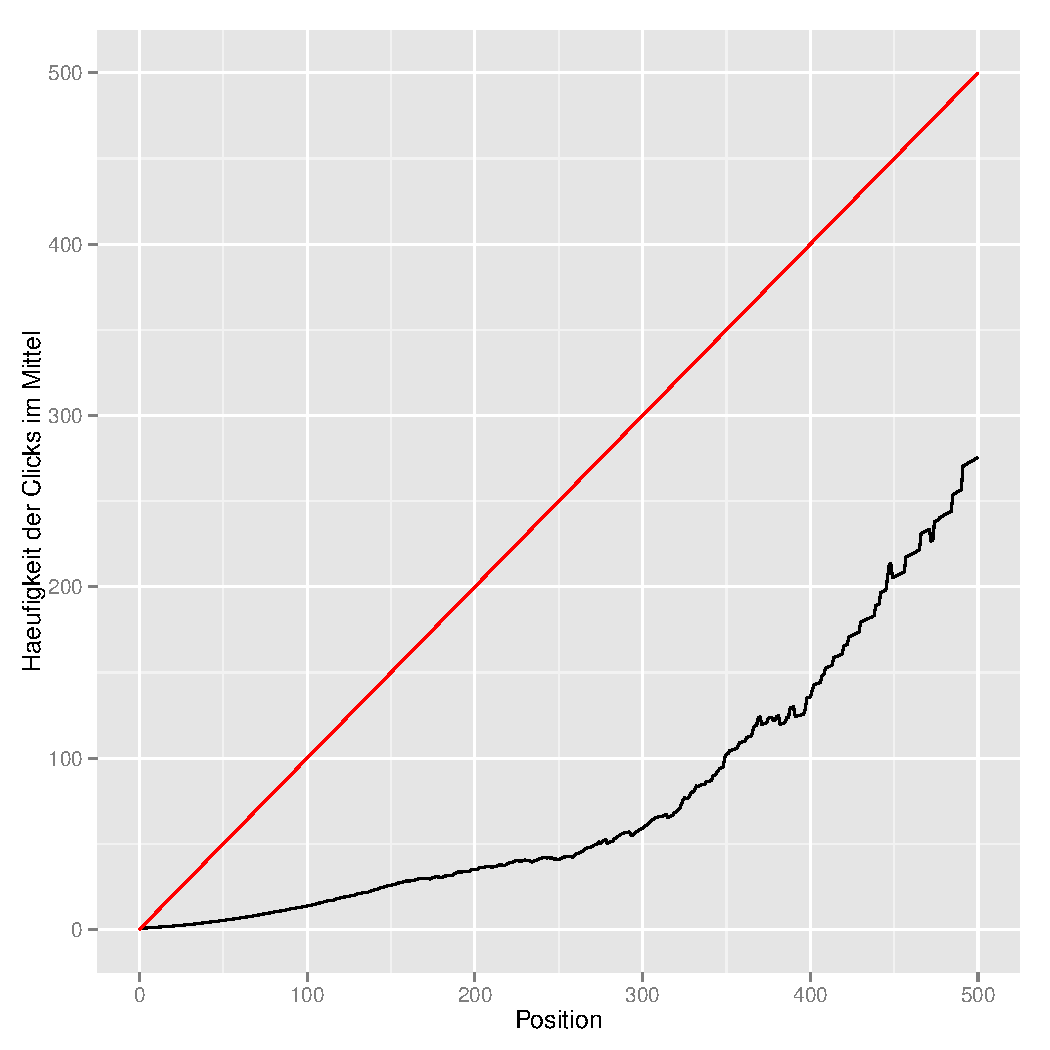
\includegraphics[scale=0.5]{clickCountSucc.pdf}
    \caption{Häufigkeit der Clicks im Mittel für jede Position}
    \label{clickCount}
\end{figure}

\subsubsection*{hasClicked}
Die Variable \textit{hasClicked} (siehe Abbildung \ref{hasClicked}) gibt für jede Position den Anteil der Funnels an, die bis dorthin mindestens einen \textit{Click} enthalten. Dieser Wert nimmt zwischen Position $1$ und Position $7$ ab. Dies ist dadurch zu erklären, dass es viele Funnels gibt, die \textit{Clicks} enthalten und deren Länge kleiner als $6$ ist. Sobald diese Funnels beendet sind, werden sie an der nächsten Position selbstverständlich nicht mehr berücksichtigt. Ab Position $7$ steigt die Kurve dann bist zur $1$ an. Ein Wert von $1$ bedeutet, dass alle Funnels bereits einen \textit{Click} hatten.
\begin{figure}[H]
    \centering
    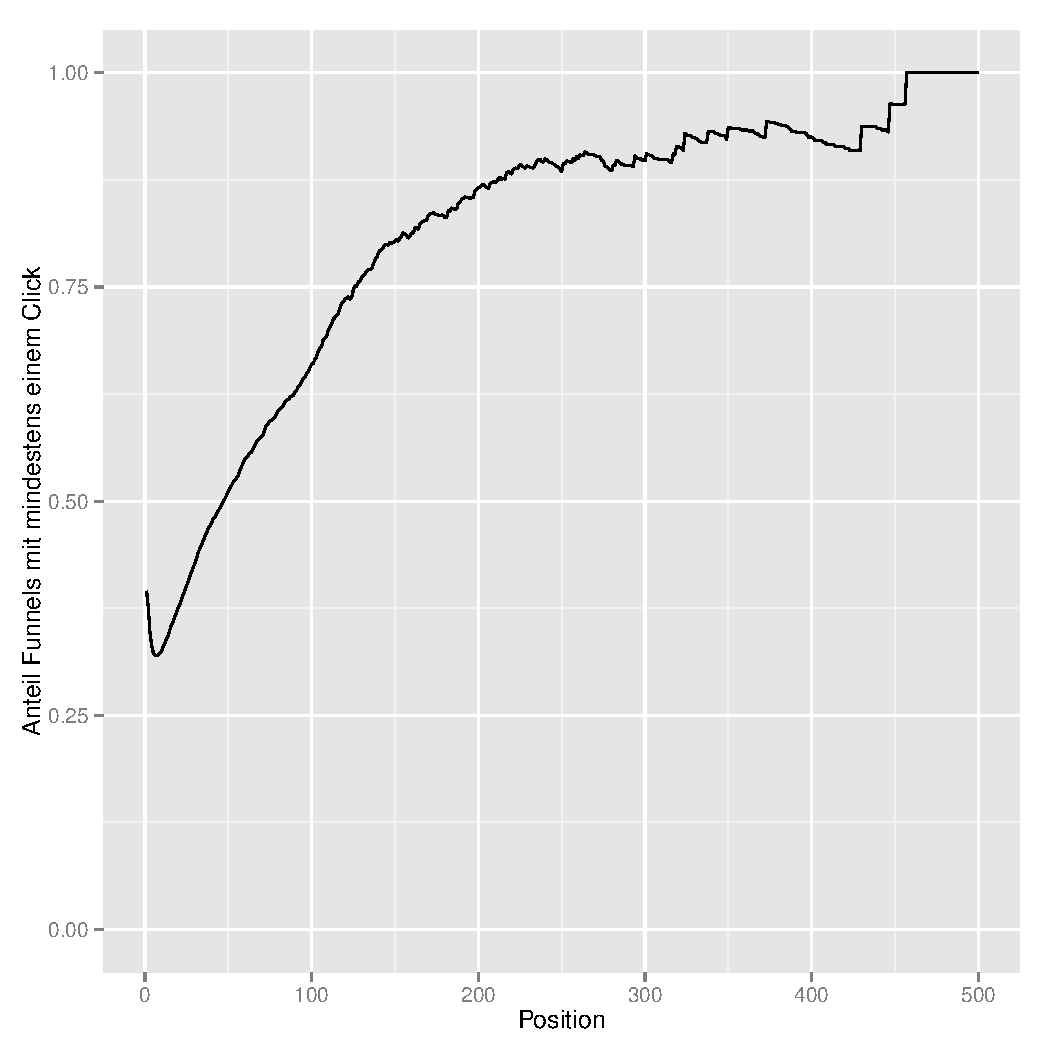
\includegraphics[scale=0.5]{hasClickedSucc.pdf}
    \caption{Anteil der Funnels mit mindestems einem Click für jede Position}
    \label{hasClicked}
\end{figure}

\subsubsection*{campaign}
Nun sollen noch die verschiedenen Kategorien des Features \textit{campagin}, das heißt die verschiedenen Werbeformen betrachtet werden. Tabelle \ref{beschreibungCampaign} enthält Erklärungen der $17$ verwendeten Kategorien.
\begin{table}[H]
  \begin{center}
		\begin{tabular}{|l|p{10cm}|}
			\hline \textbf{Kampagne} & \textbf{Beschreibung}\\ \hline
      \hline Affiliate - Partnerprogramm & Partner, die von der Interhyp AG bereitgestellte Werbemittel wie Rechner, Logo oder Banner einbinden\\
      \hline Affiliate - Rest & Partner, die einen Zinsvergleich bereitstellen, welcher das Zinsangebot der Interhyp AG mit deren Wettbewerbern im Vergleich darstellt\\ 
      \hline Direct & Potentieller Kunde gibt im Browser direkt \textit{www.interhyp.de} ein\\ 
      \hline Display & Bannerschaltungen\\
      \hline E-Mailing & Mails an Interessenten, die schon einen Antrag gestellt oder ein Infopaket angefordert hatten\\
      \hline Generic & Potentieller Kunde kommt über unbezahlten Link zur Interhyp AG\\
			\hline Kooperationen - Focus & \multirow{5}{10cm}{Individuelle Zusammenarbeiten mit größeren Partnern, die je nach Vertrag verschiedene Werbemittel auf ihrer Seite einbinden}\\
			Kooperationen - Immonet & \\
			Kooperationen - Immoscout24 & \\
			Kooperationen - Immowelt & \\
			Kooperationen - Rest & \\
			\hline Newsletter & Regelmäßige Rundschreiben\\
			\hline SEM - Brand & Bezahlte Suchergebnisse, wobei nach \textit{Interhyp} oder ähnlichem gesucht wurde\\
			\hline SEM - Remarketing & Bezahlte Suchergebnisse, wobei der potentielle Kunde bereits zuvor auf der Seite der Interhyp AG war\\
			\hline SEM - Generisch & Bezahlte Suchergebnisse, wobei nach \textit{Baufinanzierung} oder ähnlichem gesucht wurde\\
			\hline SEO & Unbezahlte Suchergebnisse\\
			\hline Social Media & Werbung, vor allem auf \textit{facebook} und \textit{gutefrage.net}\\
			\hline
    \end{tabular} 
  \end{center}
	\caption{Beschreibung der Kampagnen}\label{beschreibungCampaign}
\end{table}
Betrachtet man nur die Success Funnels genauer bezüglich ihrer Kampagnen, ist es möglich diese nach Views zu unterteilen, weil hier die Informationen vorliegen. Der Graphpanel mit Views zeigt die große Masse die Display hat und das es eine sehr schiefe Datenlage vorliegt, wenn man sie inkludiert. Mit einer relativen Häufigkeit von 84 \% überwiegt diese Werbeform schon sehr extrem. Der zweite Graphpanel ohne Views entspricht dem von der nächsten Variable und wird dort genauer erläutert. \label{campaignSucc}.
\begin{figure}[H]
    \centering
    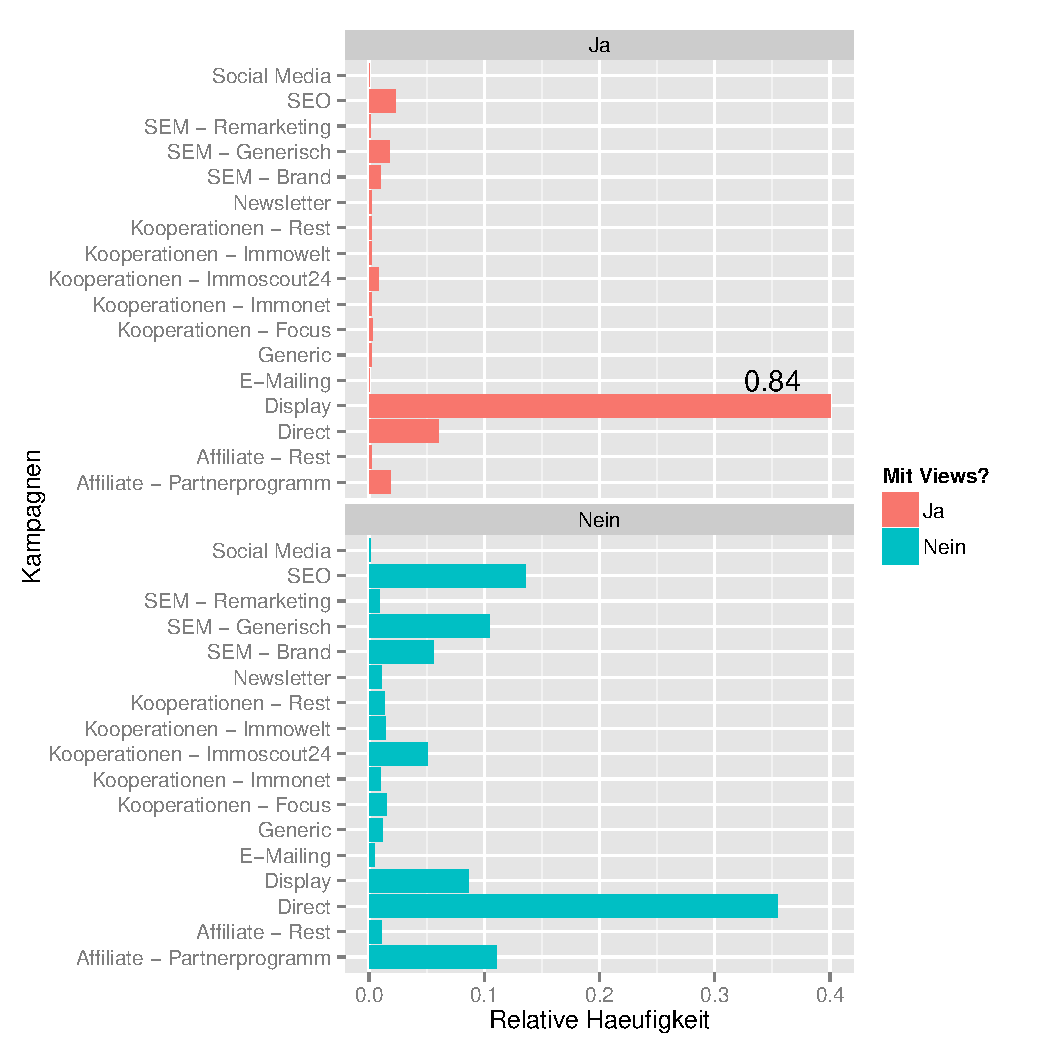
\includegraphics[scale=0.5]{campaignSucc.pdf}
    \caption{Kampagnen der konvertierten Funnels mit und ohne Views}
    \label{campaignSucc}
\end{figure}

\subsection{Vergleich von konvertierten und nicht-konvertierten Funnels}

\subsubsection*{Wochentag}
Die erste Variable die betrachtet wird , ist die Faktorvariable Wochentag des touchpoints und ist mit den Wochentagen codiert. Dazu haben wir für Success und Fail Funnels je ein separates Histogramm erstellt um einen Überblick über die Verteilung der Kontaktpunkte bezüglich der Wochentage zu erhalten. Hierbei ist anzumerken, dass es mehr Fails am Wochenende gibt und dies vor allem am Sonntag auftritt. Das heißt, es gibt  mehr Success unter der Woche. 

\begin{figure}[H]
    \centering
    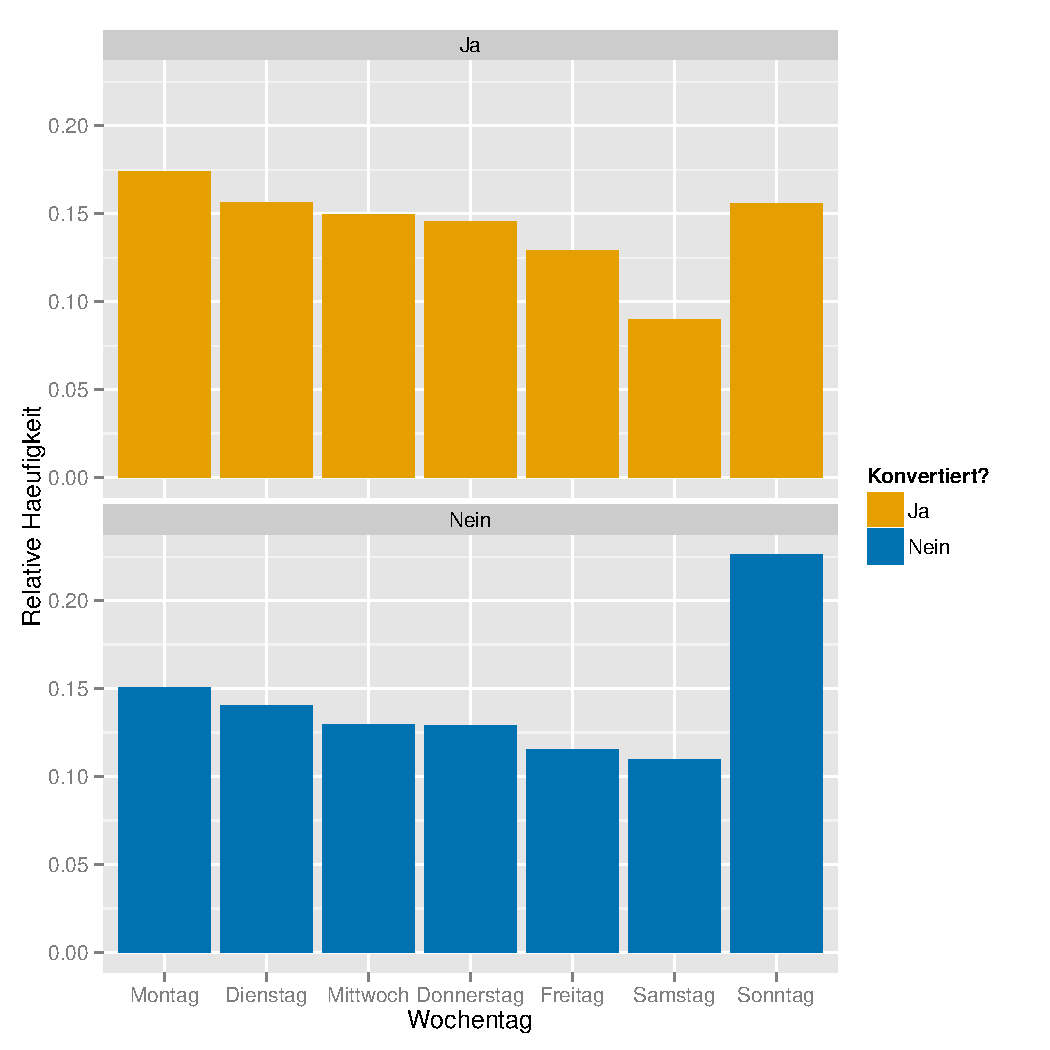
\includegraphics[scale=0.5]{weekday.pdf}
    \caption{www}
    \label{Fig_1}
\end{figure}

\subsubsection*{Uhrzeit des Kontaktpunktes}
Das nächste Histogramm wird mit der Variable hour wieder für Success und Fails getrennt erzeugt. Hour gibt die volle Stunde des touchpoints an und wurde hierzu auf die bereits verstrichen Stunde abgerundet. Daraus ergeben sich dann logischerweise Beobachtungen zwischen 0 Uhr und 23 Uhr. Zu Beginn des Tages steigt die relative Häufigkeit bis 11 Uhr an und bleibt auf auf diesem Niveau bis 21 Uhr bevor es wieder abfällt. In der Nacht sind bei weitem weniger Menschen online und deshalb liegen in dem Zeit raum zwischen 2 Uhr und 6 Uhr wenige Daten vor.
\begin{figure}[H]
    \centering
    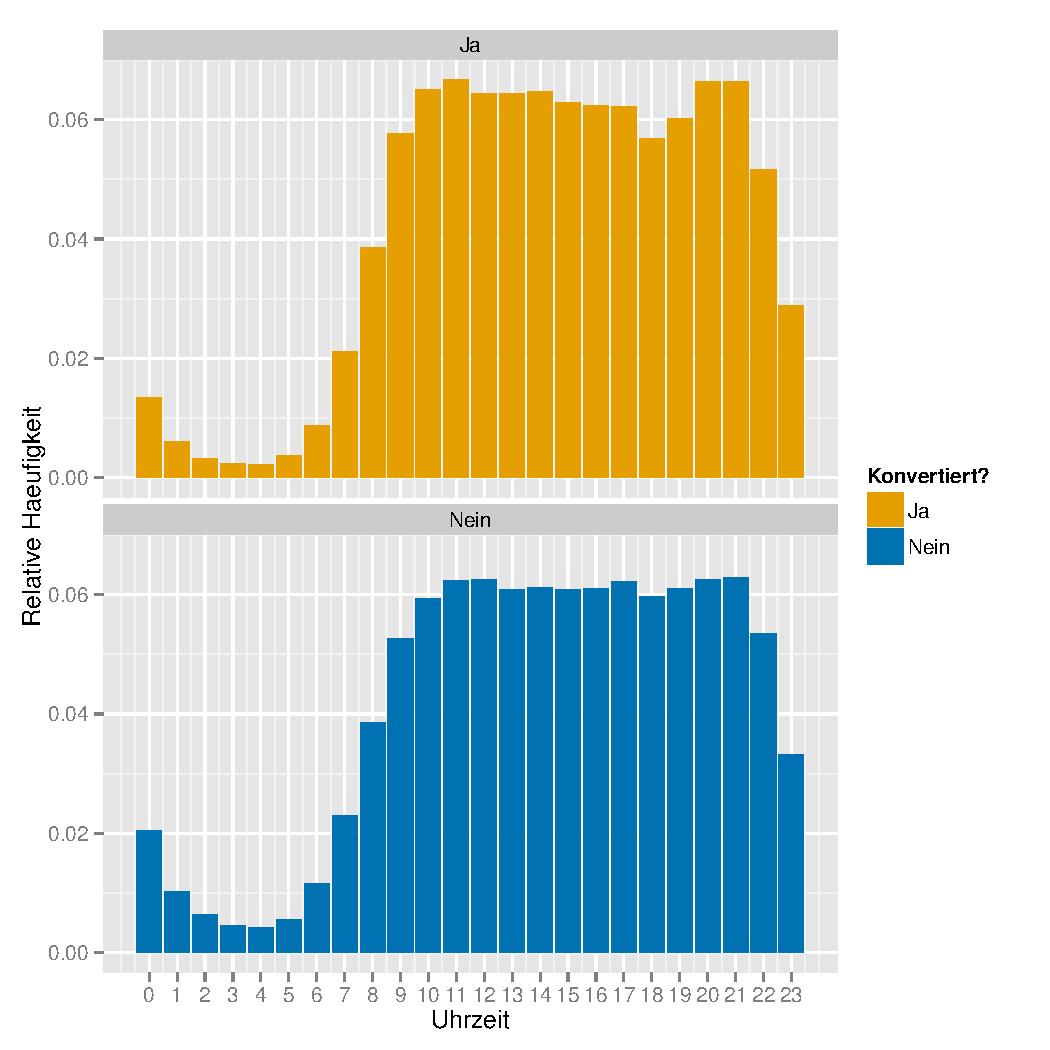
\includegraphics[scale=0.5]{hour.pdf}
    \caption{www}
    \label{Fig_2}
\end{figure}



\subsubsection*{Campaigns für Success und Fail Funnels}
 Ab hier werden die Views herausgenommen, wie es in \ref{datenlage} erläutert wird. Unterscheidet man nun die Kampagnen nach konvertierten und nichtkonvertierten Funnels, sieht man , dass es bei den Success Funnels sehr häufig der Direkteinstig benutzt worden ist. Bei den Fails wurden hauptsächlich Display und die Affiliate Partnerprogramme benützt. Die hohe relative Häufigkeit bei Affiliate kann aber 
auch auf einen Trackingfehler zurückzuführen sein.

    \begin{figure}[H]
        \centering
        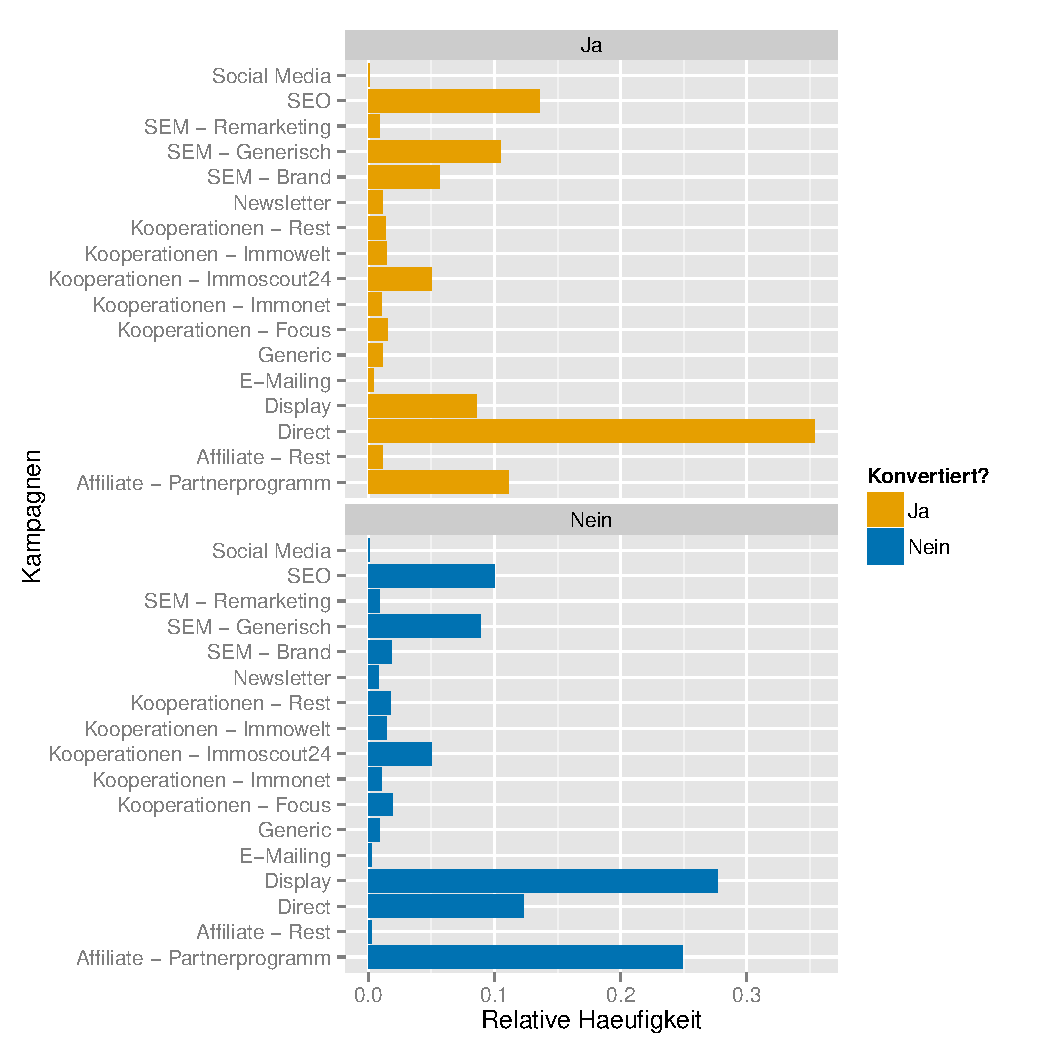
\includegraphics[scale=0.5]{campaign.pdf}
        \caption{Funnels breakdown campaigns}
        \label{Fig_6}
    \end{figure}
    



\subsubsection*{Länge der Funnels}
funnelLength gibt die Anzahl von touchpoints in einem Funnel an.Der Hauptteil der Fail Funnels hat nur einen Kontaktpunkt und daraus ergibt sich eine längere funnel Länge für Konvertierte Funnels. Dafür spricht auch der Mean und Median von Success mit 57 und 8 vs. 8 und 2 bei den Fails. 


\begin{figure}[H]
    \centering
    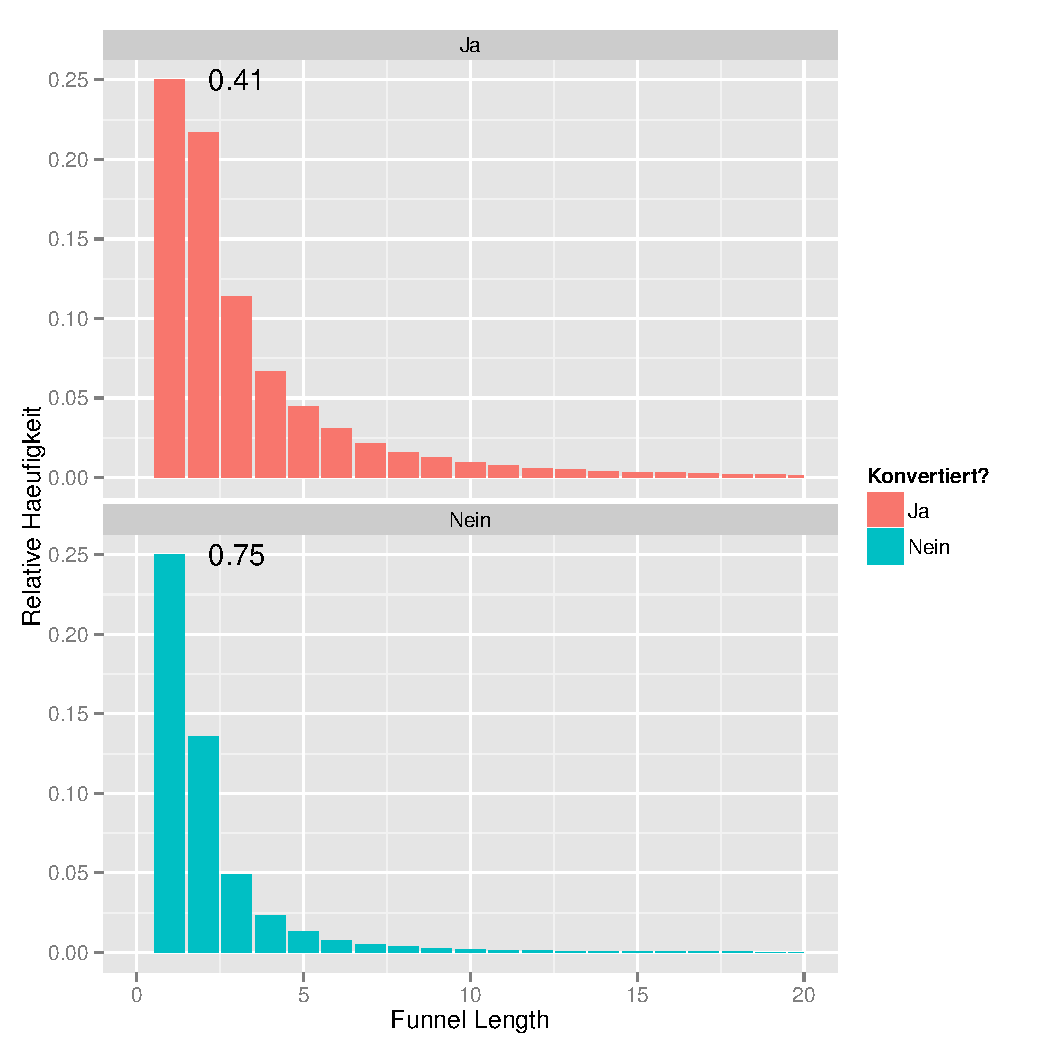
\includegraphics[scale=0.5]{funnelLength_First.pdf}
    \caption{Länge der Funnels}
    \label{Fig_7}
\end{figure}






\subsubsection*{Dauer des Funnels}
Um die Beobachtungstage in Tagen zu betrachten , wird timeSinceFirst des letzten Kontaktpunktes analysiert. Wie vorhin schon erwähnt gibt es sehr viel Fail Funnels mit nur einem Touchpoint, deswegen ist hier auch die Beobachtungsdauer mit weniger als einem Tag die stärkste Gruppe. Im Einklang mit den vorherigen Ergebnissen, ergibt sich für die Success Funnels in den anderen Gruppen jeweils eine höhere Relative Häufigkeit und somit mit steigender Beobachtungsdauer eine häufigere Konvertierung.
Diese These stützen der Mittelwert für die konvertierten Funnels liegt mit 21.1 Tage und bei den nicht konvertierten mit 5.3 Tagen
Desweiteren ist eine wöchentliche Periodizität zu erkennen, da in Abstand von 7 Tagen relative Häufigkeit wieder zunimmt und sonst stetig fällt.  Auf Rücksprache , ist ein mögliche Erklärung dafür auf die verstärkt am Wochenende vorkommenden Focus und Spiegel Kampagnen zurückzuführen.


\begin{figure}[H]
    \centering
    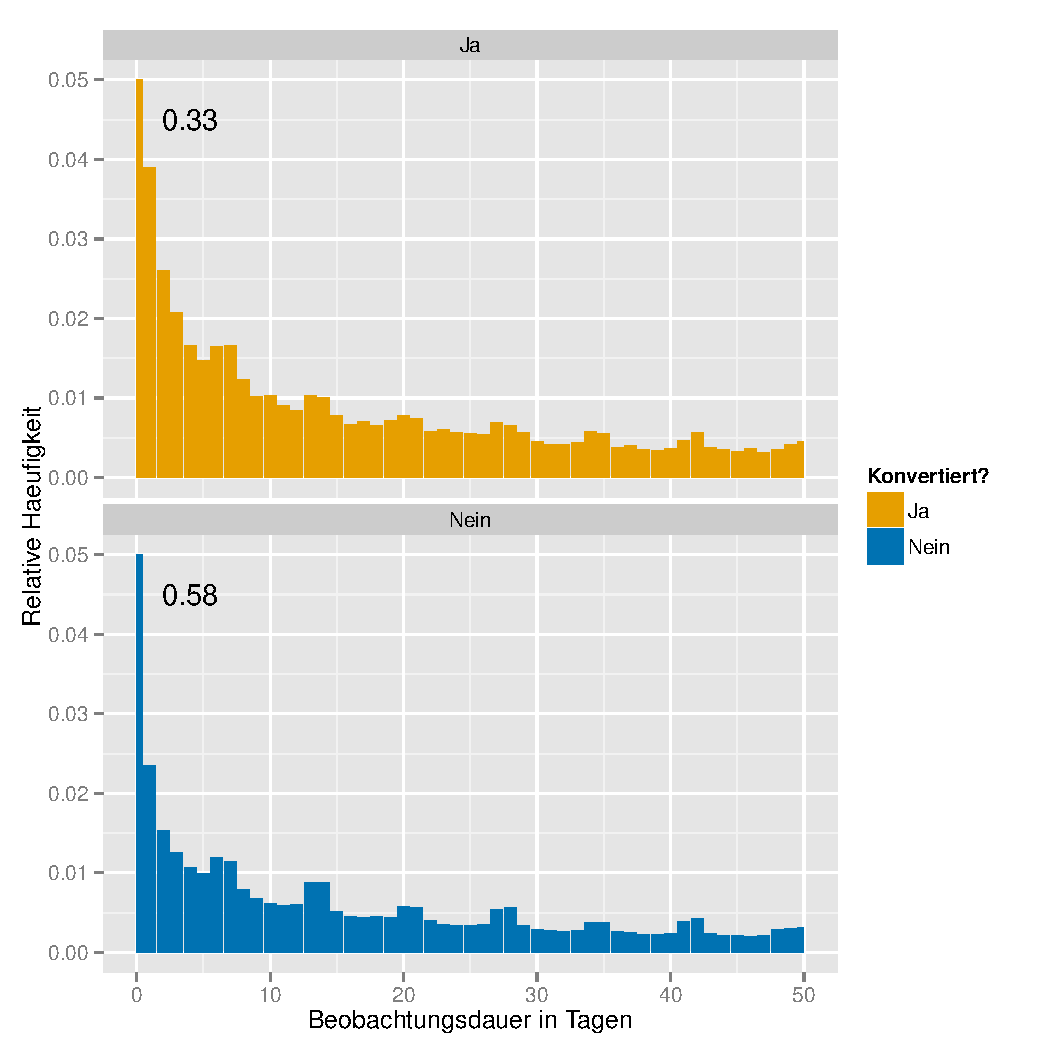
\includegraphics[scale=0.5]{timeSinceFirst_Last.pdf}
    \caption{Beobachtungsdauer der Funnels in Tagen}
    \label{Fig_8}
\end{figure}




\subsubsection*{Zeitlicher Abstand des aktuellen und vorherigen touchpoints}
TimeSinceLast gibt die verstrichene Zeit zweier aufeinander folgender Touchpoints an und man erkennt wieder die wöchentliche Periodizität wie bei den Beobachtungsdauern. Hier ist auffällig, dass die Fails nur bei einer erneuten Kontaktierung innerhalb von 24 Stunden eine höhere relative Häufigkeit haben. 

\begin{figure}[H]
    \centering
    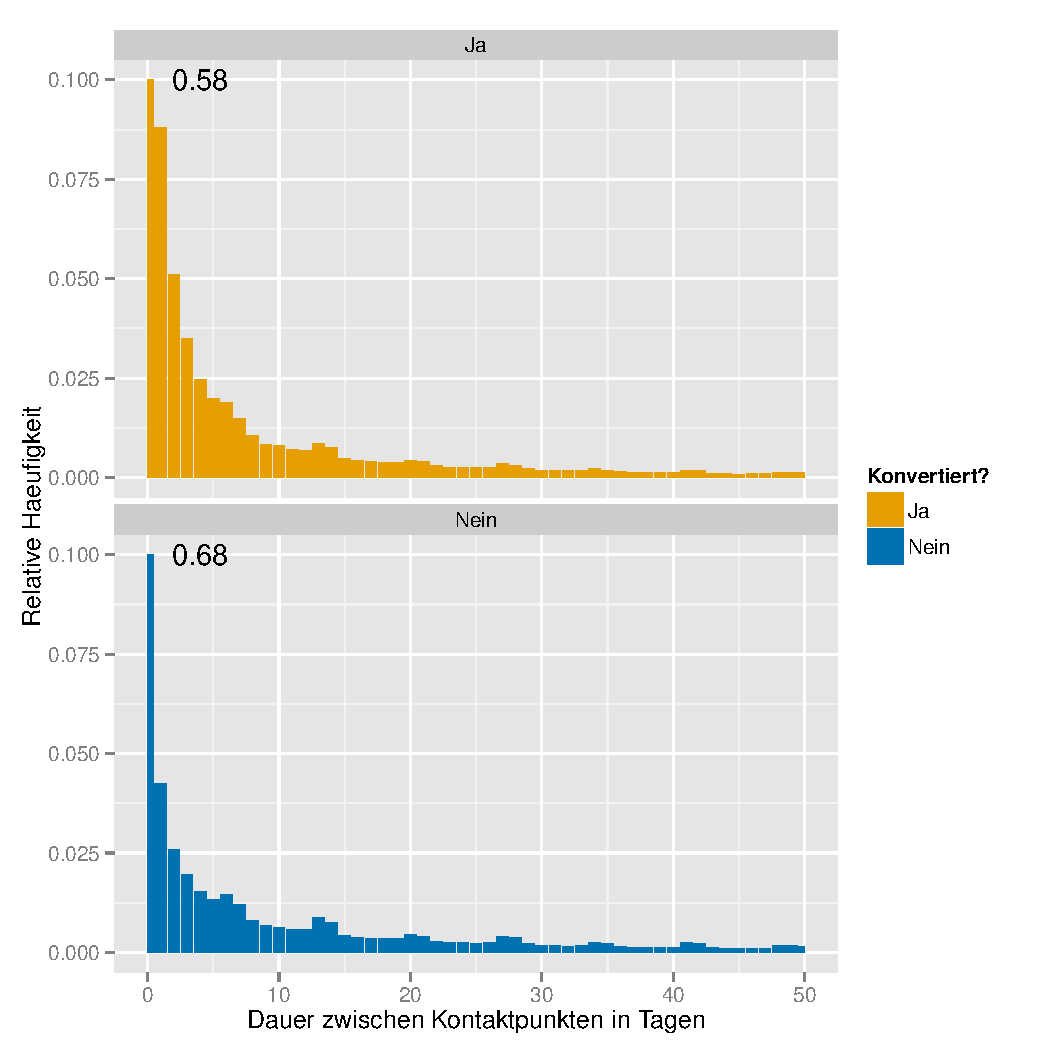
\includegraphics[scale=0.5]{timeSinceLast.pdf}
    \caption{Zeitlicher Abstand des aktuellen und vorherigen touchpoints}
    \label{Fig_9}
\end{figure}


\subsubsection*{Frequenz der Kontaktpunkte}
Berechnet man den Quotienten aus funnelLength und timeSincefirst, umgerechnet auf Stunden, ergibt sich sowas wie eine "Frequenz" der Kontaktpunkte. Diese Variable soll uns Aufschluss über die Anzahl an Kontaktpunkten geben die ein potentieller Kunde in einem gewissen Zeitraum hat und uns Information zu einer eventuellen Übersättigung geben. Für jede funnelLenght wurde hierzu ein Boxplot erstellt und aus Übersichtgründen wurden hier nur die Längen drei bis 25 betrachtet. 
Nicht konvertierte Funnels haben häufiger eine höhere Frequenz, dass heißt die haben mehr Touchpoints als konvertierte in der gleichen Zeit. Auch der Median liegt bei allen funnelLengths über den der konvertierten. Im Schnitt haben alle konvertierten Funnels eine Frequenz von 96.89 im Vergleich zu 267.17 bei den nicht konvertierten. Das bedeutet die Nicht konvertierten werden 3 mal so oft im gleichen Zeitraum kontaktiert. Die spricht schon eher für eine Übersättigung. Zudem nicht die Frequenz mit steigender funnel Länge ab, wobei dies für die Success Funnels schon wesentlich früher Eintritt.
Das bedeutet  dass eine längere Kontaktierung in längeren Abschnitten auf einen höheren Erfolg für ein Konvertierung deuten.\\


- Man könnte sagen, dass der häufige Kontakt am Anfang erwünscht ist und mit zunehmender Dauer nicht?
    \begin{figure}[H]
        \centering
    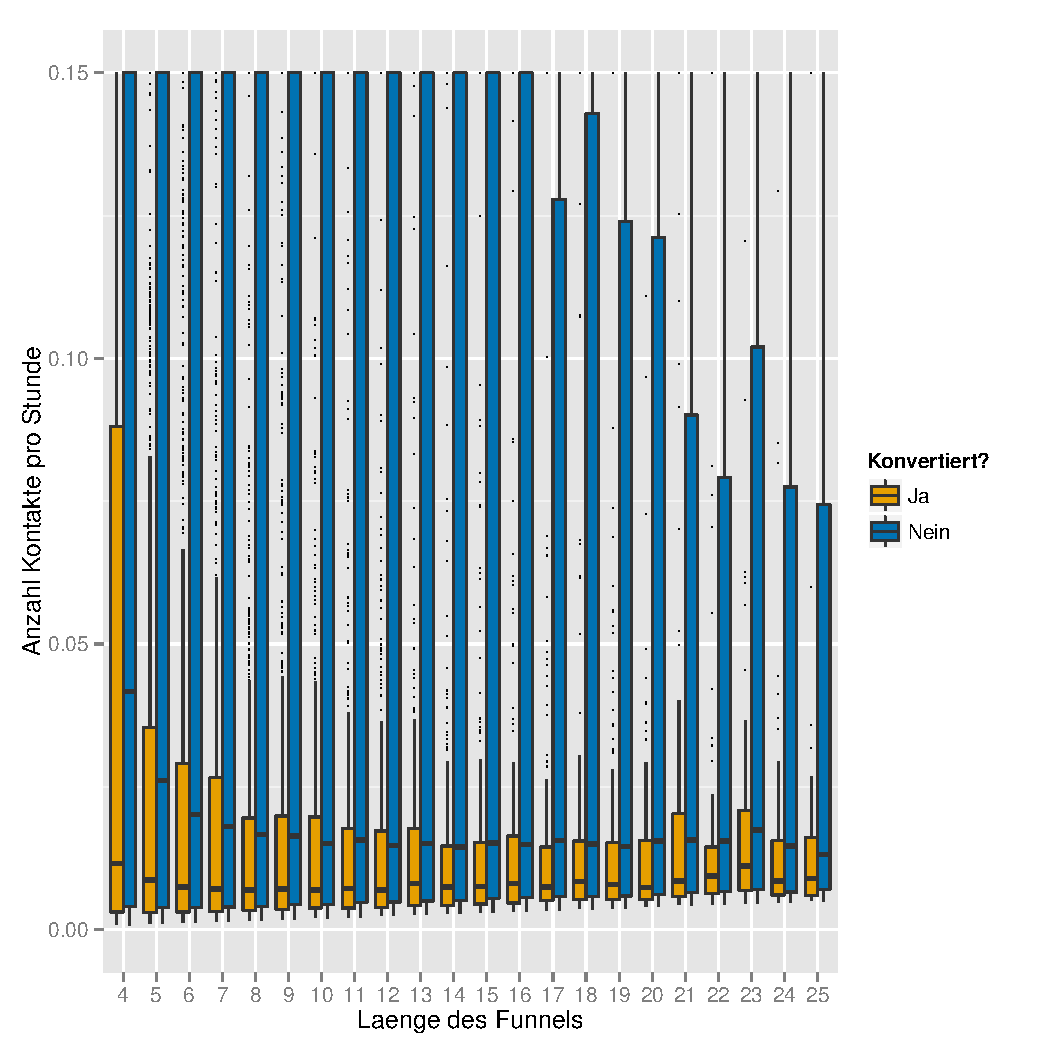
\includegraphics[scale=0.5]{freq.pdf}
    \caption{Frequenz der Kontaktpunkte}
    \label{Fig_10}
    \end{figure}
    













































